

\section{Experiments}
\label{sec:experiment}


In this section, we provide results and insights from the experimentation, to answer our research questions.





\begin{figure}[t!]
  \centering
   \begin{subfigure}[b]{0.24\textwidth}
         \centering
         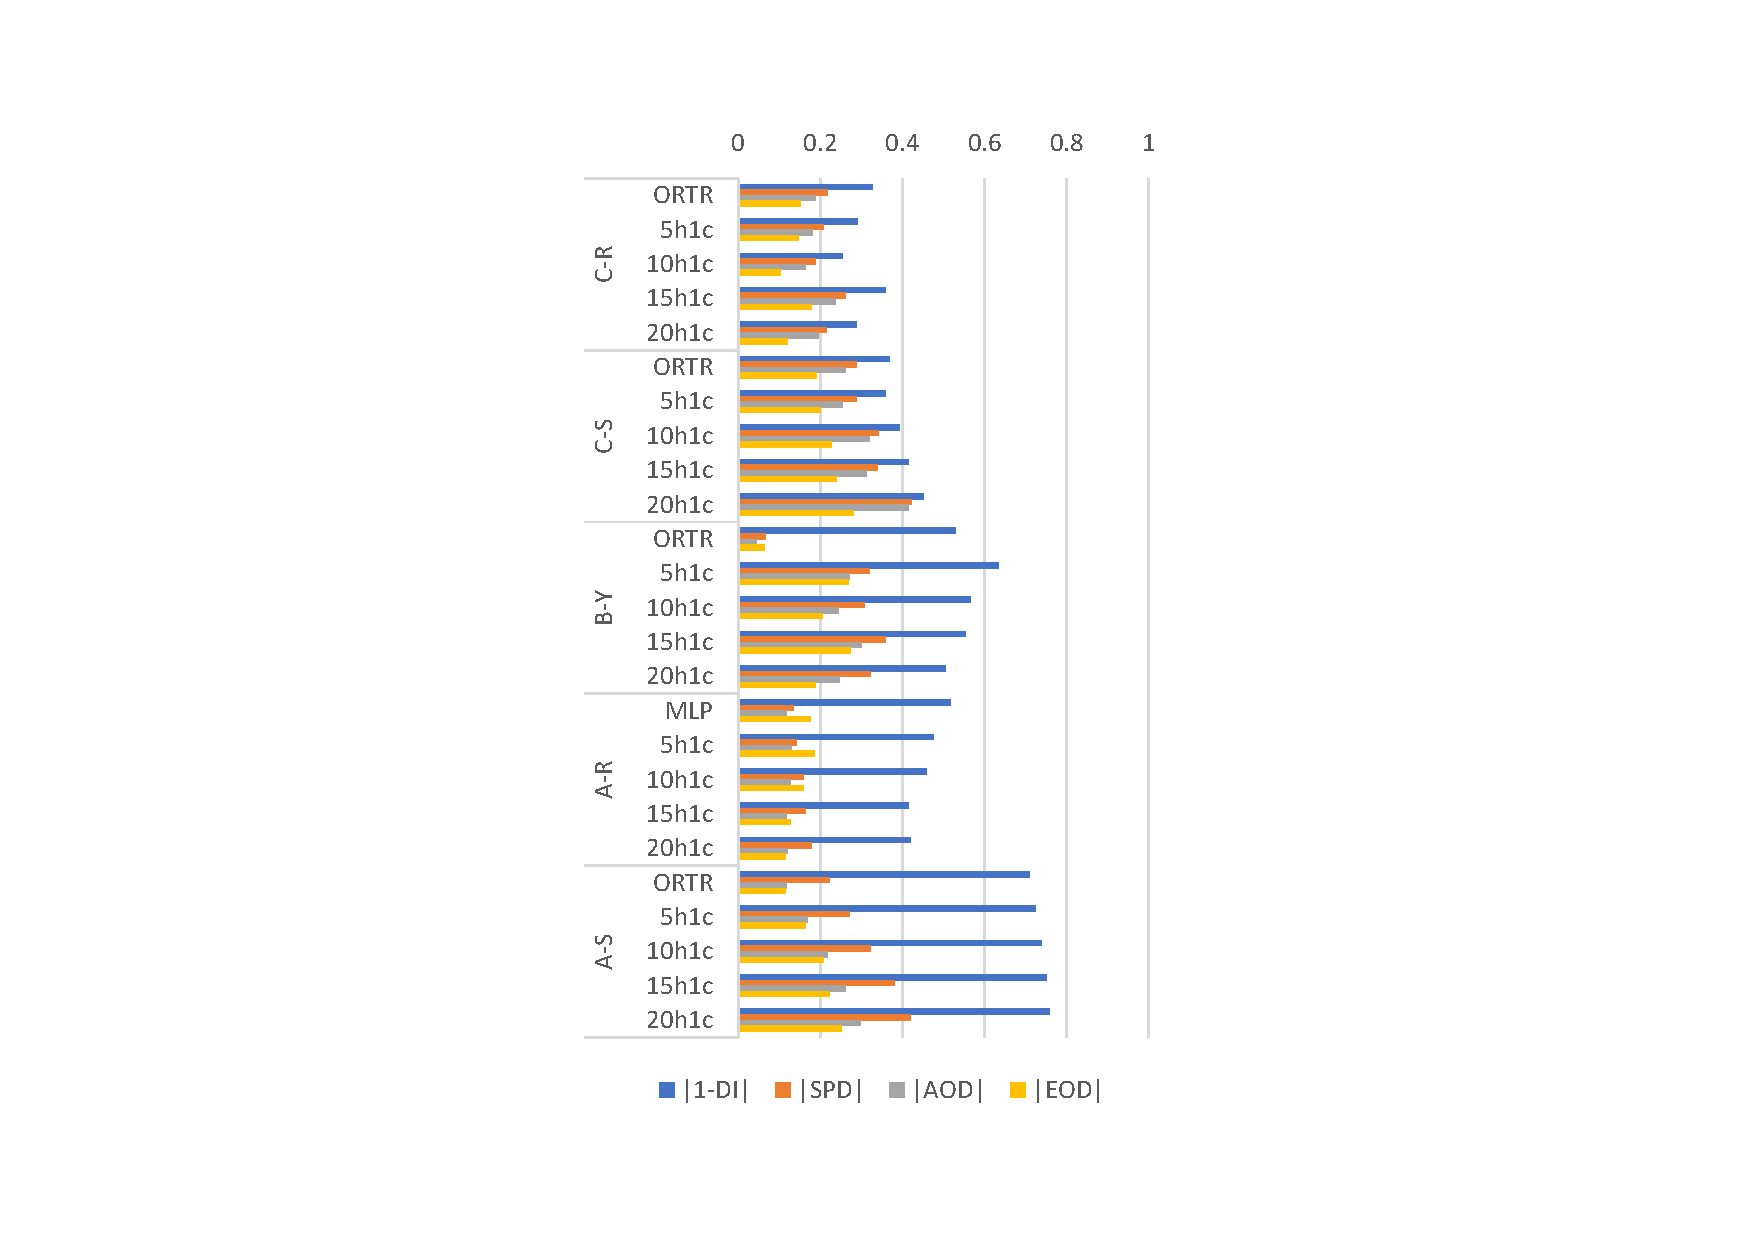
\includegraphics[width=\textwidth]{assets/rq1-fairness-1slice-vertical.pdf}
         \caption{Fairness metrics for \\ 5/10/15/20 shards one slice
         }
         \label{fig:rq1-fairness-1slice}
 \end{subfigure}
    \begin{subfigure}[b]{0.24\textwidth}
         \centering
         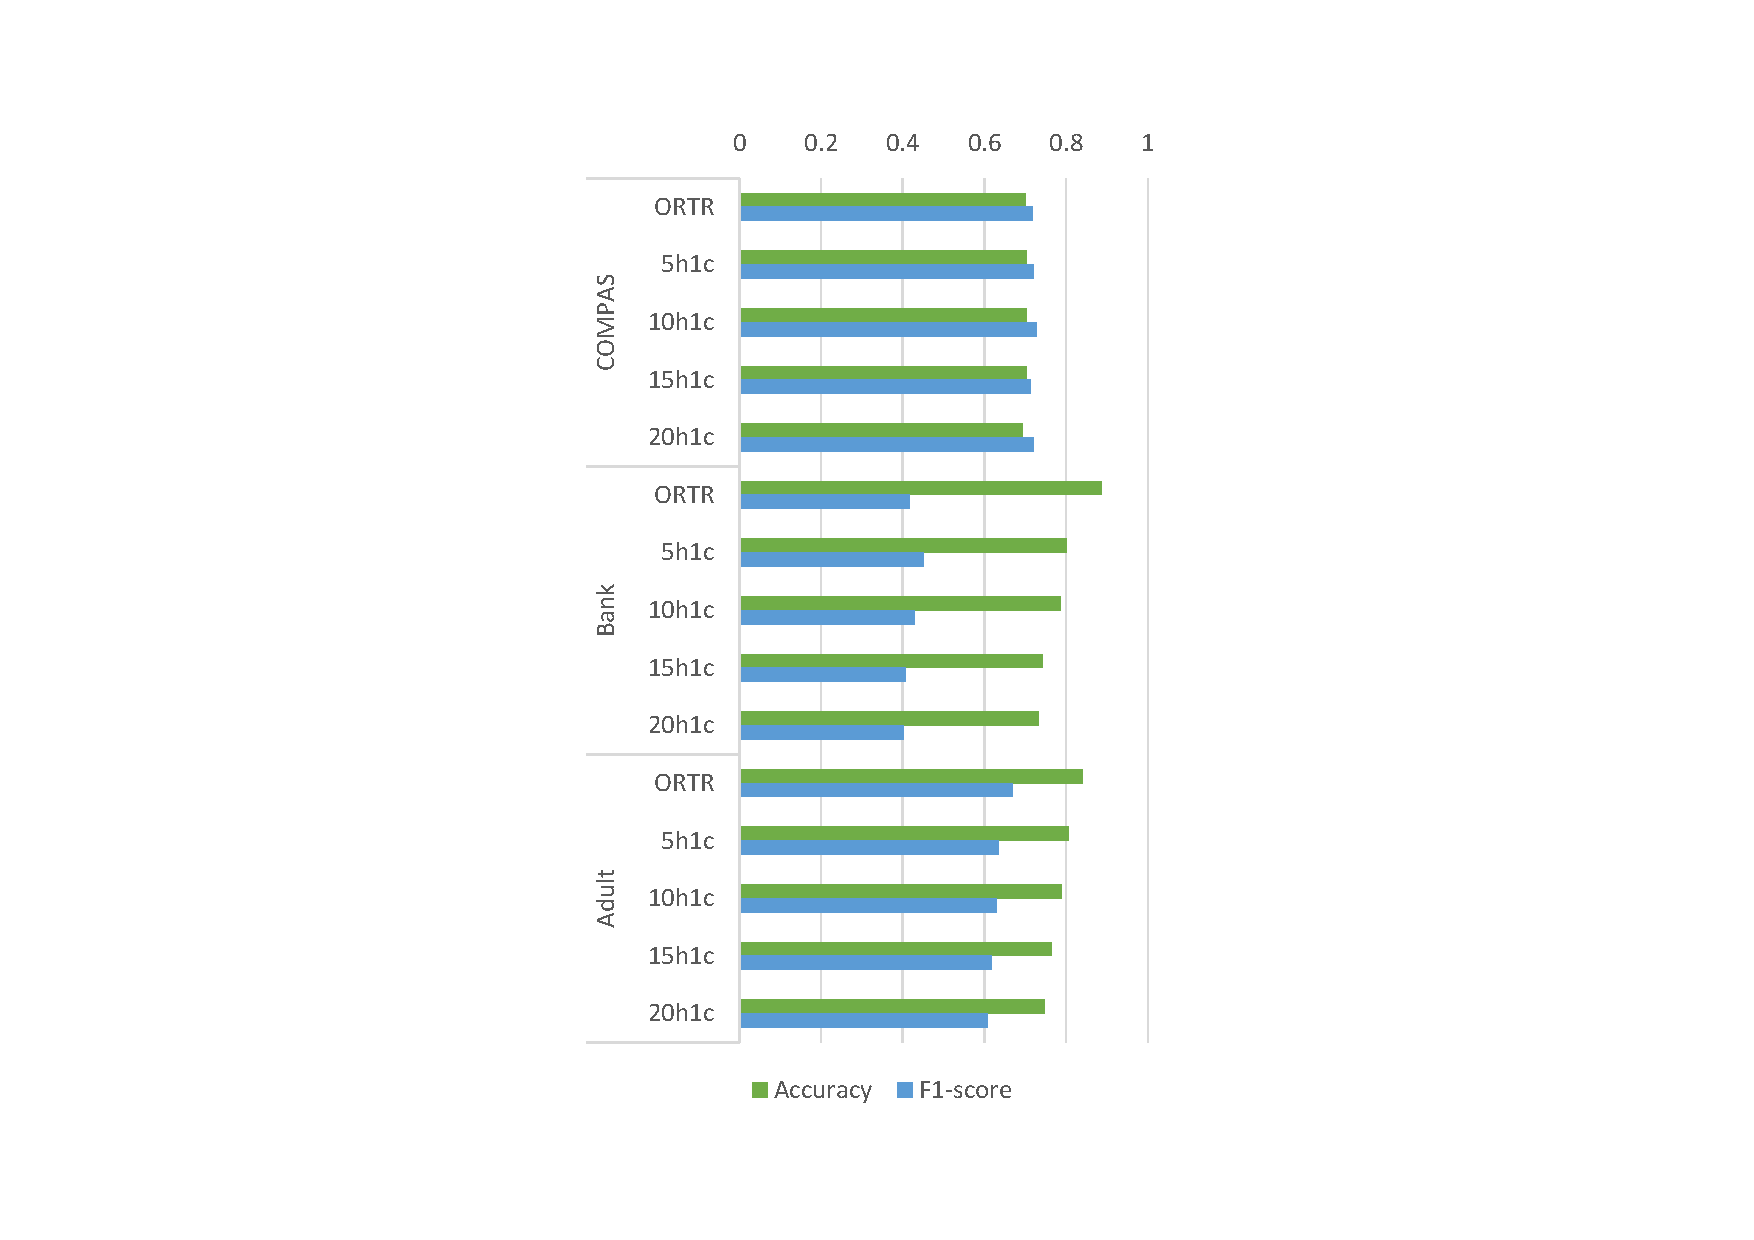
\includegraphics[width=\textwidth]{assets/rq1-performance-1slice-vertical.pdf}
         \caption{Performance metrics for \\ 5/10/15/20 shards one slice}
         \label{fig:rq1-performance-1slice}
 \end{subfigure}



 \begin{subfigure}[b]{0.24\textwidth}
         \centering
         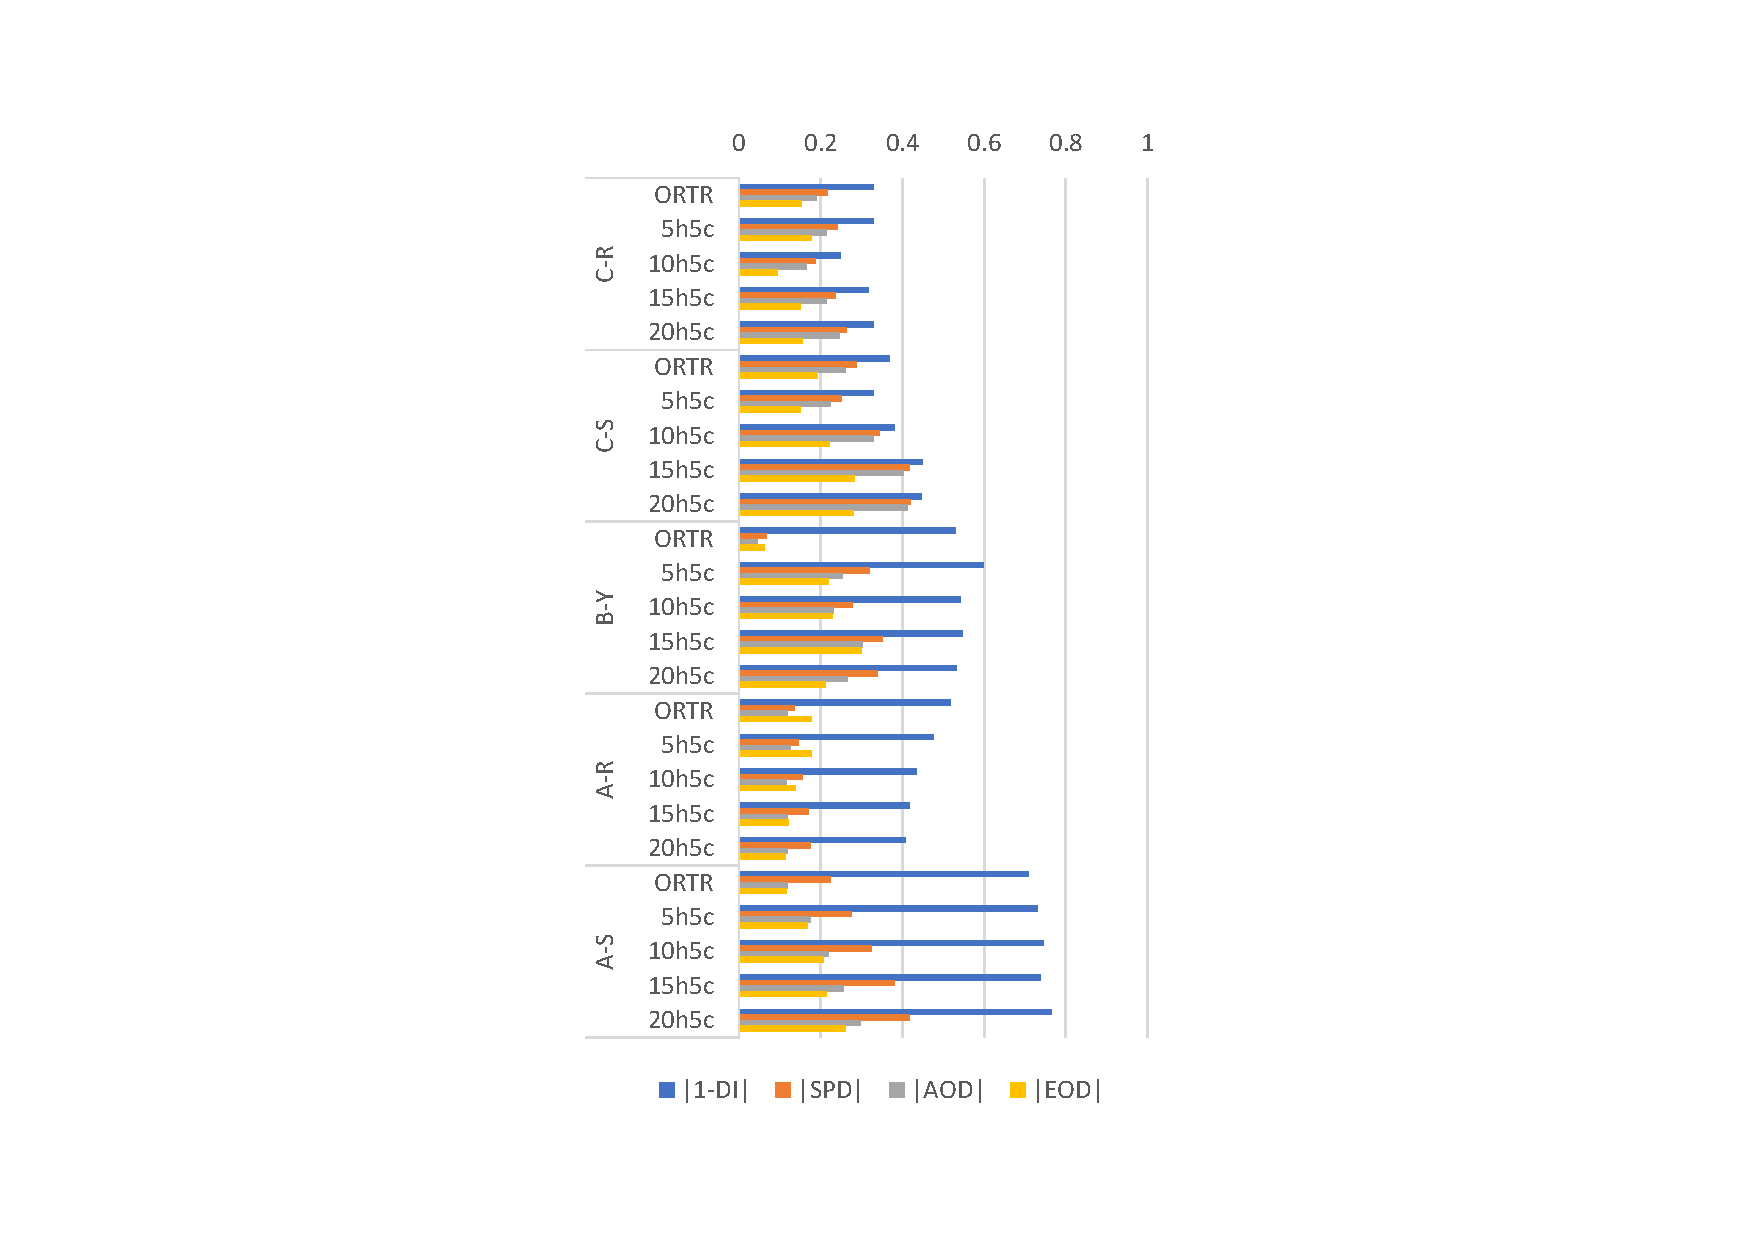
\includegraphics[width=\textwidth]{assets/rq1-fairness-5slice-vertical.pdf}
         \caption{Fairness metrics for \\ 5/10/15/20 shards five slices}
         \label{fig:rq1-fairness-5slice}
 \end{subfigure}
    \begin{subfigure}[b]{0.24\textwidth}
         \centering
         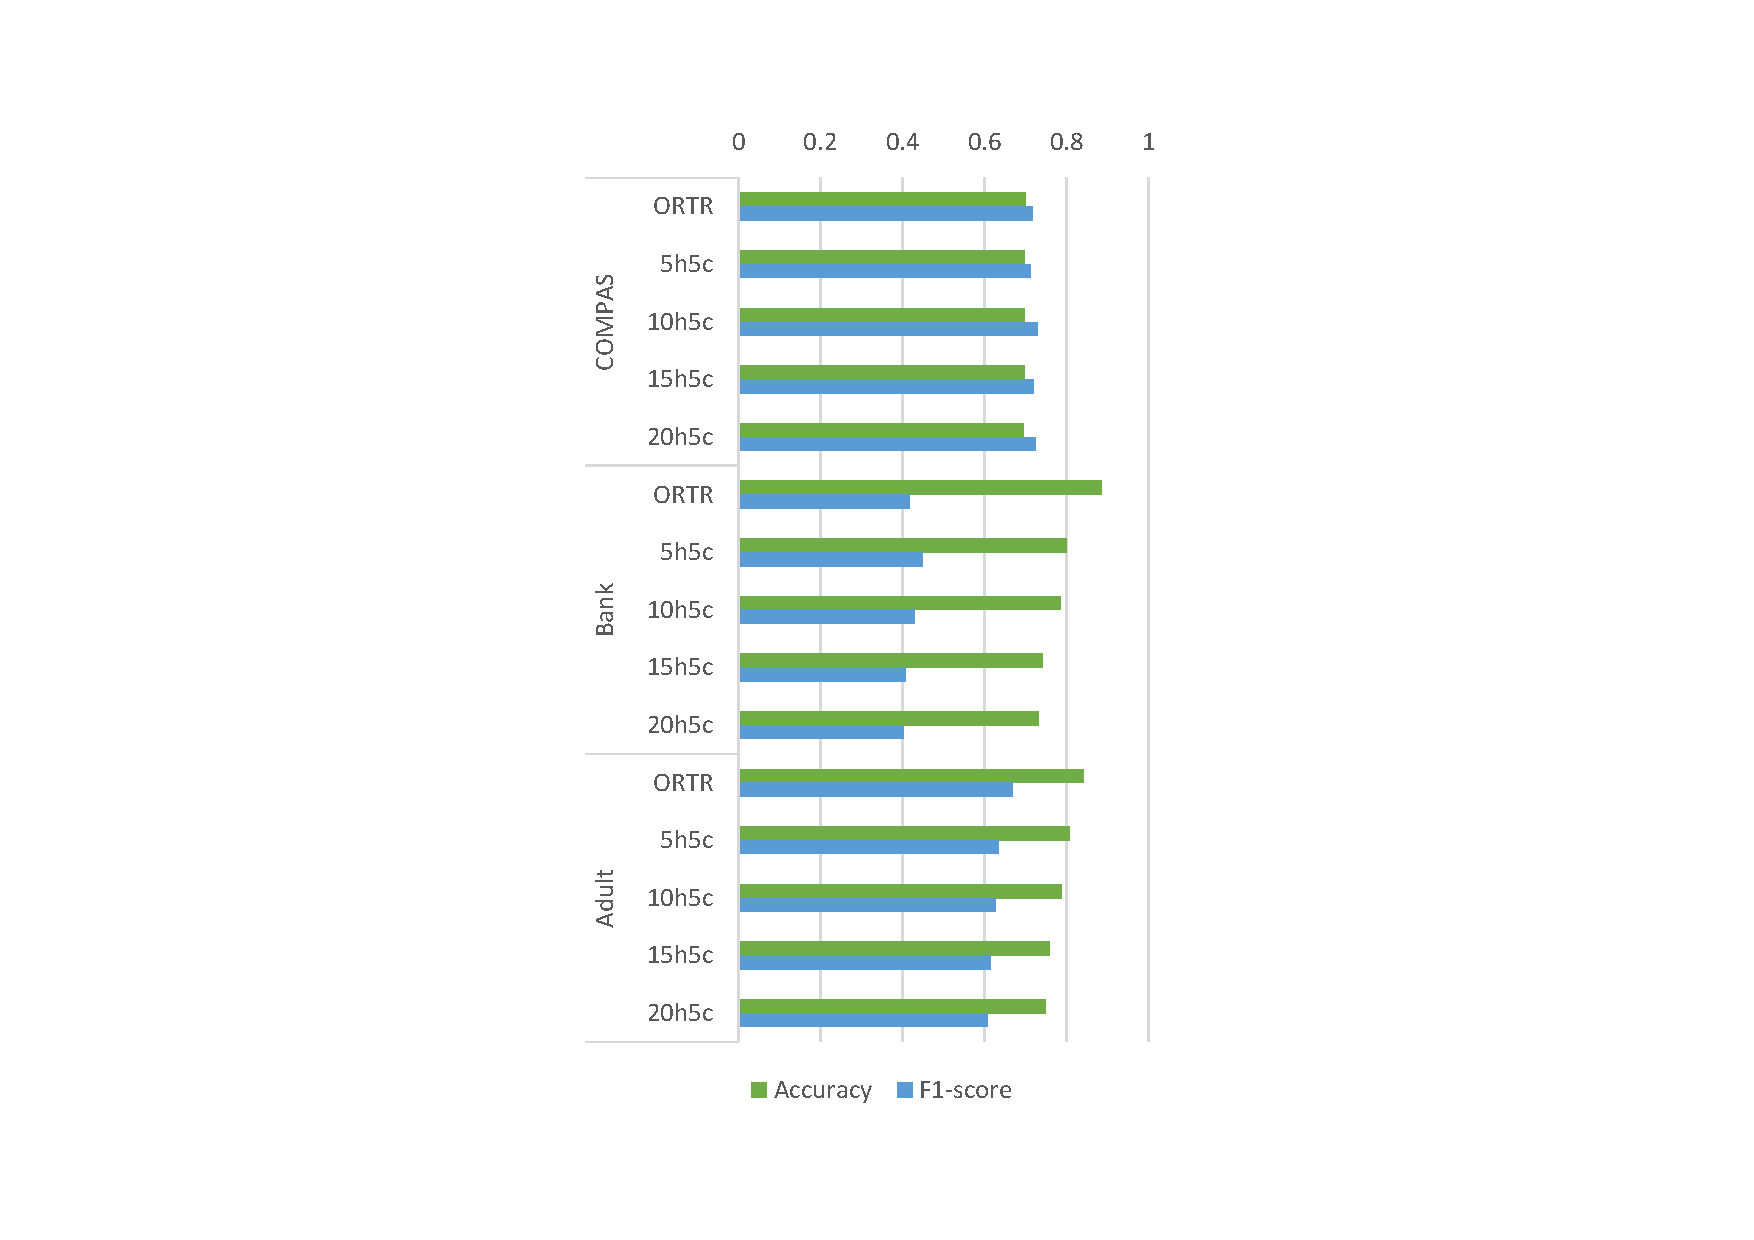
\includegraphics[width=\textwidth]{assets/rq1-performance-5slice-vertical.pdf}
         \caption{Performance metrics for \\ 5/10/15/20 shards five slices}
         \label{fig:rq1-performance-5slice}
 \end{subfigure}
  \caption{Fairness (the smaller, the better) and performance (the higher, the better) evaluation results of SISA with different shards (5/10/15/20h) and slices (1/5/10c)}
  \label{fig:rq1}
\end{figure}

\begin{figure*}[t!]
  \centering
  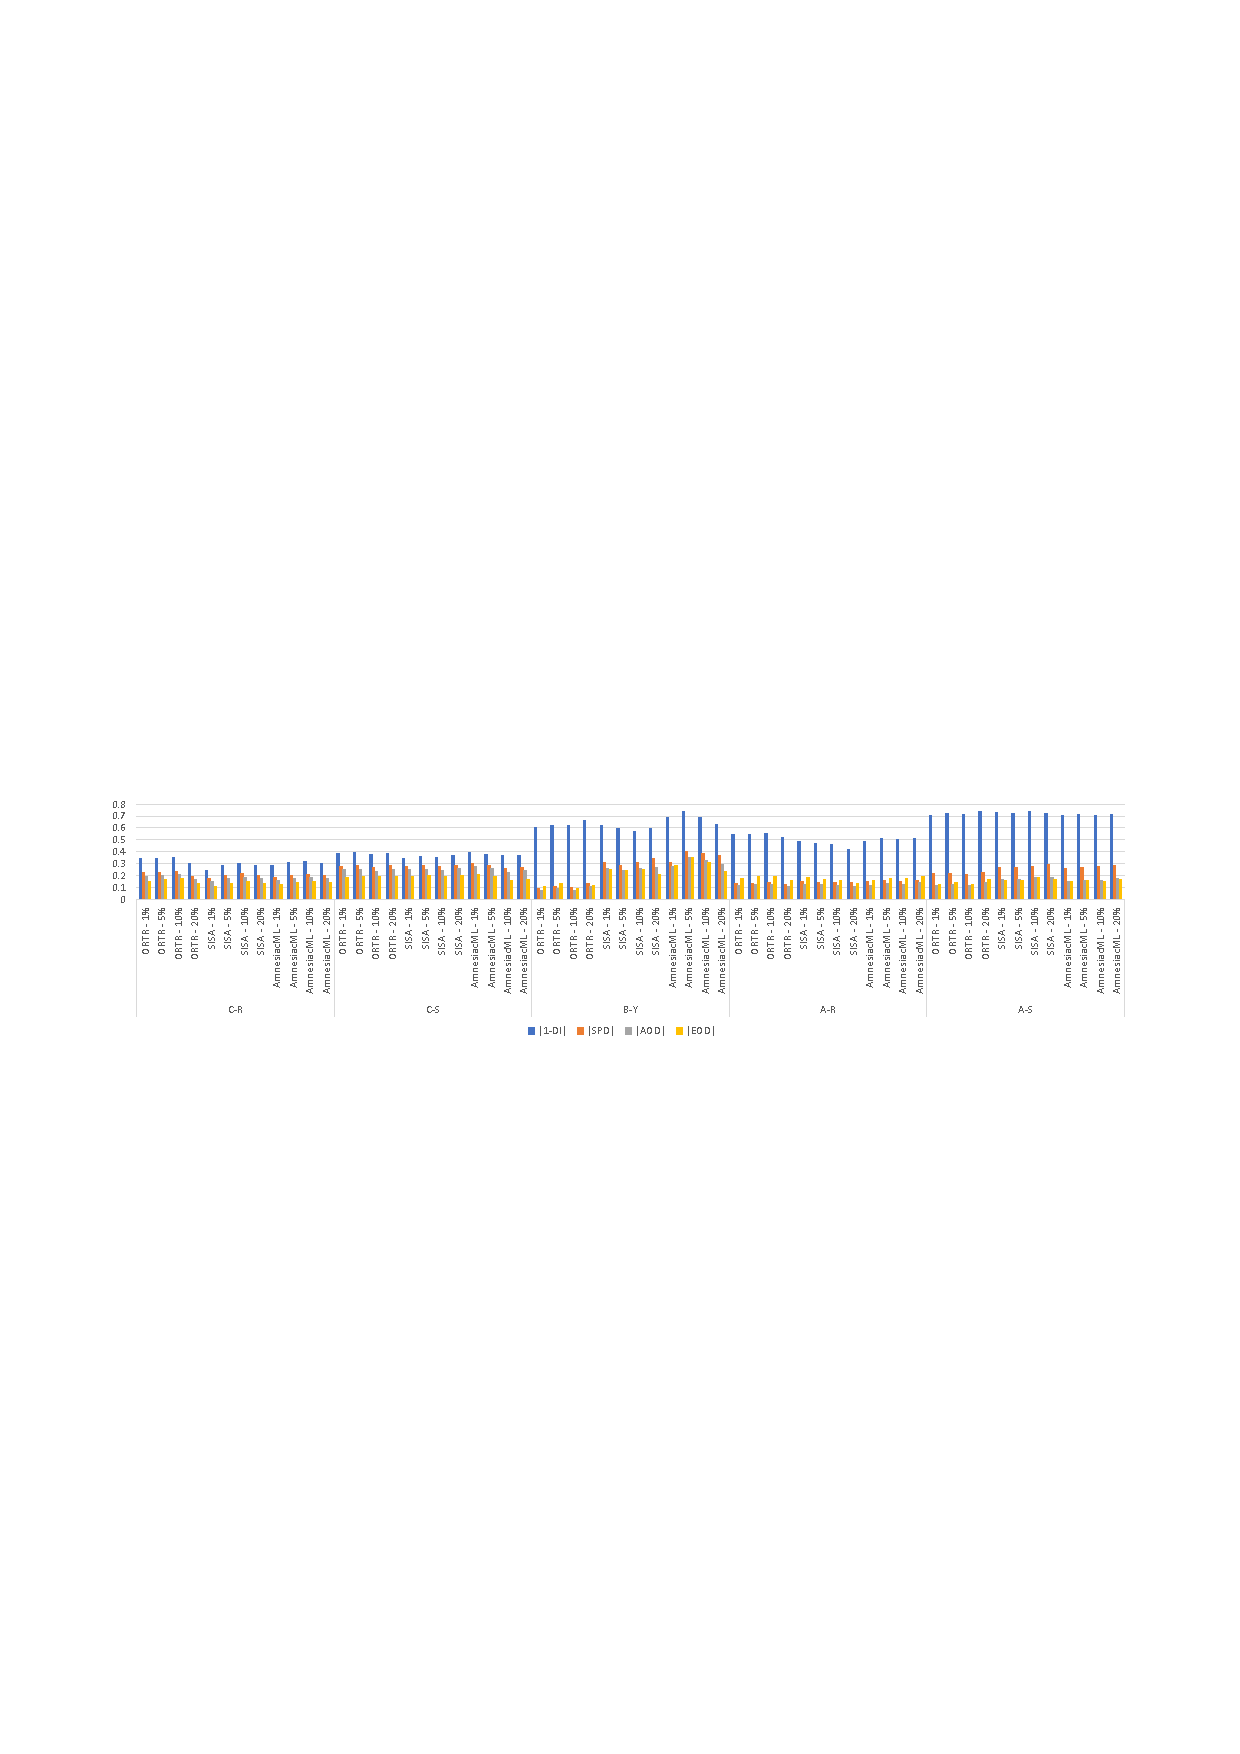
\includegraphics[width=1.0\textwidth]{assets/rq2-bar-chart.pdf}
  \caption{Fairness (the smaller, the better) evaluation results of different training methods after uniform data deletion under various deletion proportions.}
  \label{fig:rq2-bar-chart}
\end{figure*}

\begin{figure*}[t!]
  \centering
  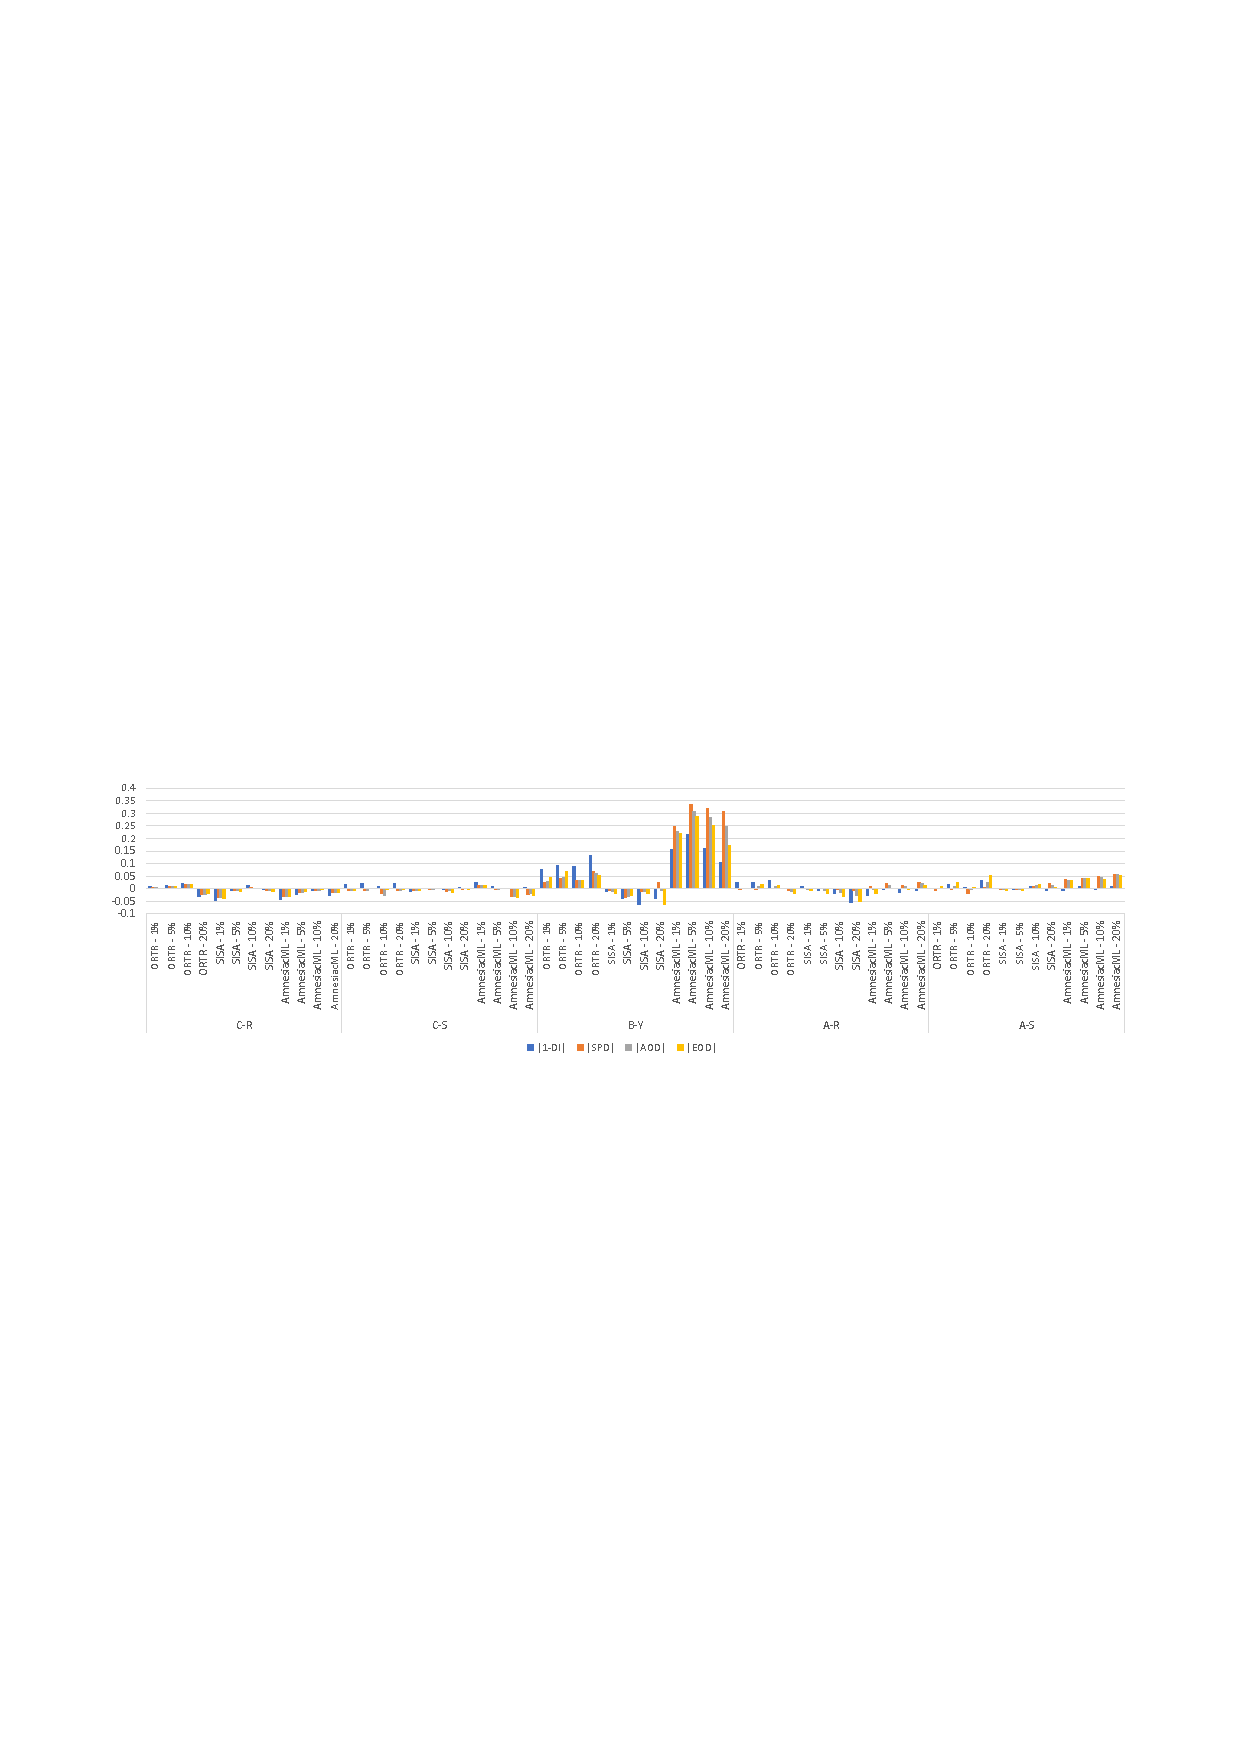
\includegraphics[width=1.0\textwidth]{assets/rq2-fairness-diff.pdf}
  \caption{Difference of fairness between before and after the deletion. Value 0 indicates no fairness change, while positive values and negative values indicate worsen fairness and improved fairness respectively. 
  }
  \label{fig:rq2-fairness-diff}
\end{figure*}

\begin{flushleft}


\noindent \textbf{RQ1: (Initial training) What are the impacts of machine unlearning methods on fairness before the ``\textit{right to be forgotten}'' requests arrive?}
\end{flushleft}


The exact machine unlearning methods, such as SISA, modify how data is fed into machine learning models, affecting the fairness of these models before RTBF is requested, i.e., initial training. 
This research question is aimed to understand the impact of
machine unlearning methods on fairness in initial training. Specifically, we compare SISA with ORTR, a na\"ive approach built based on a MLP model. Note that the approximate machine unlearning methods, such as AmnesiacML, only update the ML models' parameters without modifying their architecture. We therefore ignore AmnesiacML in this research question. 

We evaluate the impact of SISA and ORTR on fairness across different numbers of shards (5, 10, 15, 20) and numbers of slices (1, 5). We execute the experiments on three different datasets, such as Adult, Bank, and COMPAS. For ease of observation, we denote Adult, Bank, and COMPAS as \textit{A}, \textit{B}, and \textit{C}, respectively. \textit{Sex}, \textit{Race}, and \textit{Age}, which are the sensitive features, are represented as \textit{S}, \textit{R}, and \textit{Y}, respectively.
The number of shards and the number of slices are represented as \textit{h} and \textit{c}, respectively. 
For example, given 1,000 instances, \textit{5h5c} means these instances are split into five shards. Each shard is then further split into five slices. In the end, each shard contains 200 instances and each slice includes 40 instances.


Figure~\ref{fig:rq1-fairness-1slice} shows the fairness evaluation results of SISA initial training with 5/10/15/20 shards and one slice. The baseline is ORTR. We can see that for some datasets and features, the $|1-\textrm{DI}|$ value gets better when the number of shards increases, including \textit{B-Y} and \textit{A-R}, while for \textit{C-S} and \textit{A-S} the value gets worse when the number of shards increases. Similarly, for other metrics, the trends are not always one way along the increasing number of shards. Although there are some tendencies within each dataset, overall across all datasets, we cannot come up with an interpretation towards any outstanding fairness impact from the SISA method and its number of shards.



In terms of performance, there is degradation of less than 10\% in accuracy for Adult and Bank datasets, while there is no apparent degradation for the COMPAS dataset. This could be because the COMPAS dataset is much smaller than the Adult and Bank datasets and has fewer useful features, making it easier to converge and less likely to experience performance degradation from data partitioning.



The fairness evaluation results of SISA at initial training with five slices are shown in Figure~\ref{fig:rq1-fairness-5slice}. Comparing the fairness between one slice and five slices, we find no noticeable difference across all fairness metrics. We have the similar observation on performance metrics shown in Figure~\ref{fig:rq1-performance-1slice} and Figure~\ref{fig:rq1-performance-5slice}, and this is expectedly identical to what was reported in the SISA paper \cite{sisa}.

\begin{tcolorbox}During initial training, no significant fairness impacts are observed from using machine unlearning methods, such as SISA. In addition, compared with ORTR, SISA has performance degradation on larger datasets.
\end{tcolorbox}



\begin{flushleft}
\textbf{RQ2: (Uniform distribution) What are the impacts of machine unlearning methods on fairness when the deleted data has uniform distribution?}
\end{flushleft}




A uniform data deletion strategy assumes that every instance has an equal possibility of being removed from trained models. In this research question, we want to explore how much these machine unlearning methods impact fairness when the deleted data is in uniform distribution.

For this research question, we employ a range of deletion rates from small to large (1\%, 5\%, 10\%, 20\%) chosen from the statistics~\cite{rtbf5years}. 
For SISA, we apply its default setting (i.e., \textit{5h1c}).
For AmnesiacML, we train its model according to the requirements in the paper~\cite{amnesiac}.



Figure~\ref{fig:rq2-bar-chart} presents the results of fairness in various deletion proportions. We see that there is no clear trend indicating which methods achieve better results across all datasets (i.e., Adult, Bank, and COMPAS) and sensitive features (\textit{Sex}, \textit{Race}, and \textit{Age}). Figure~\ref{fig:rq2-fairness-diff} shows the difference in fairness before and after applying the deletion strategy. It indicates that AmnesiacML is likely to be prone to fairness loss caused by this deletion strategy, while SISA is the most robust. However, the difference in fairness between before and after data deletion is unclear in Adult and COMPAS datasets. The main reason is that the deleted data is in uniform distribution, i.e., each instance has an equal probability of being removed from trained models, leading to similar fairness results in this setting. We also see that all methods have a relatively large variation in fairness on the Bank dataset. The reason is that this dataset is highly imbalanced compared to other datasets, such as Adult and COMPAS. Specifically, among 45,211 instances, only 963 instances (2.13\%) are labeled as negative instances in the Bank dataset.


\begin{figure*}[htbp]
  \centering
  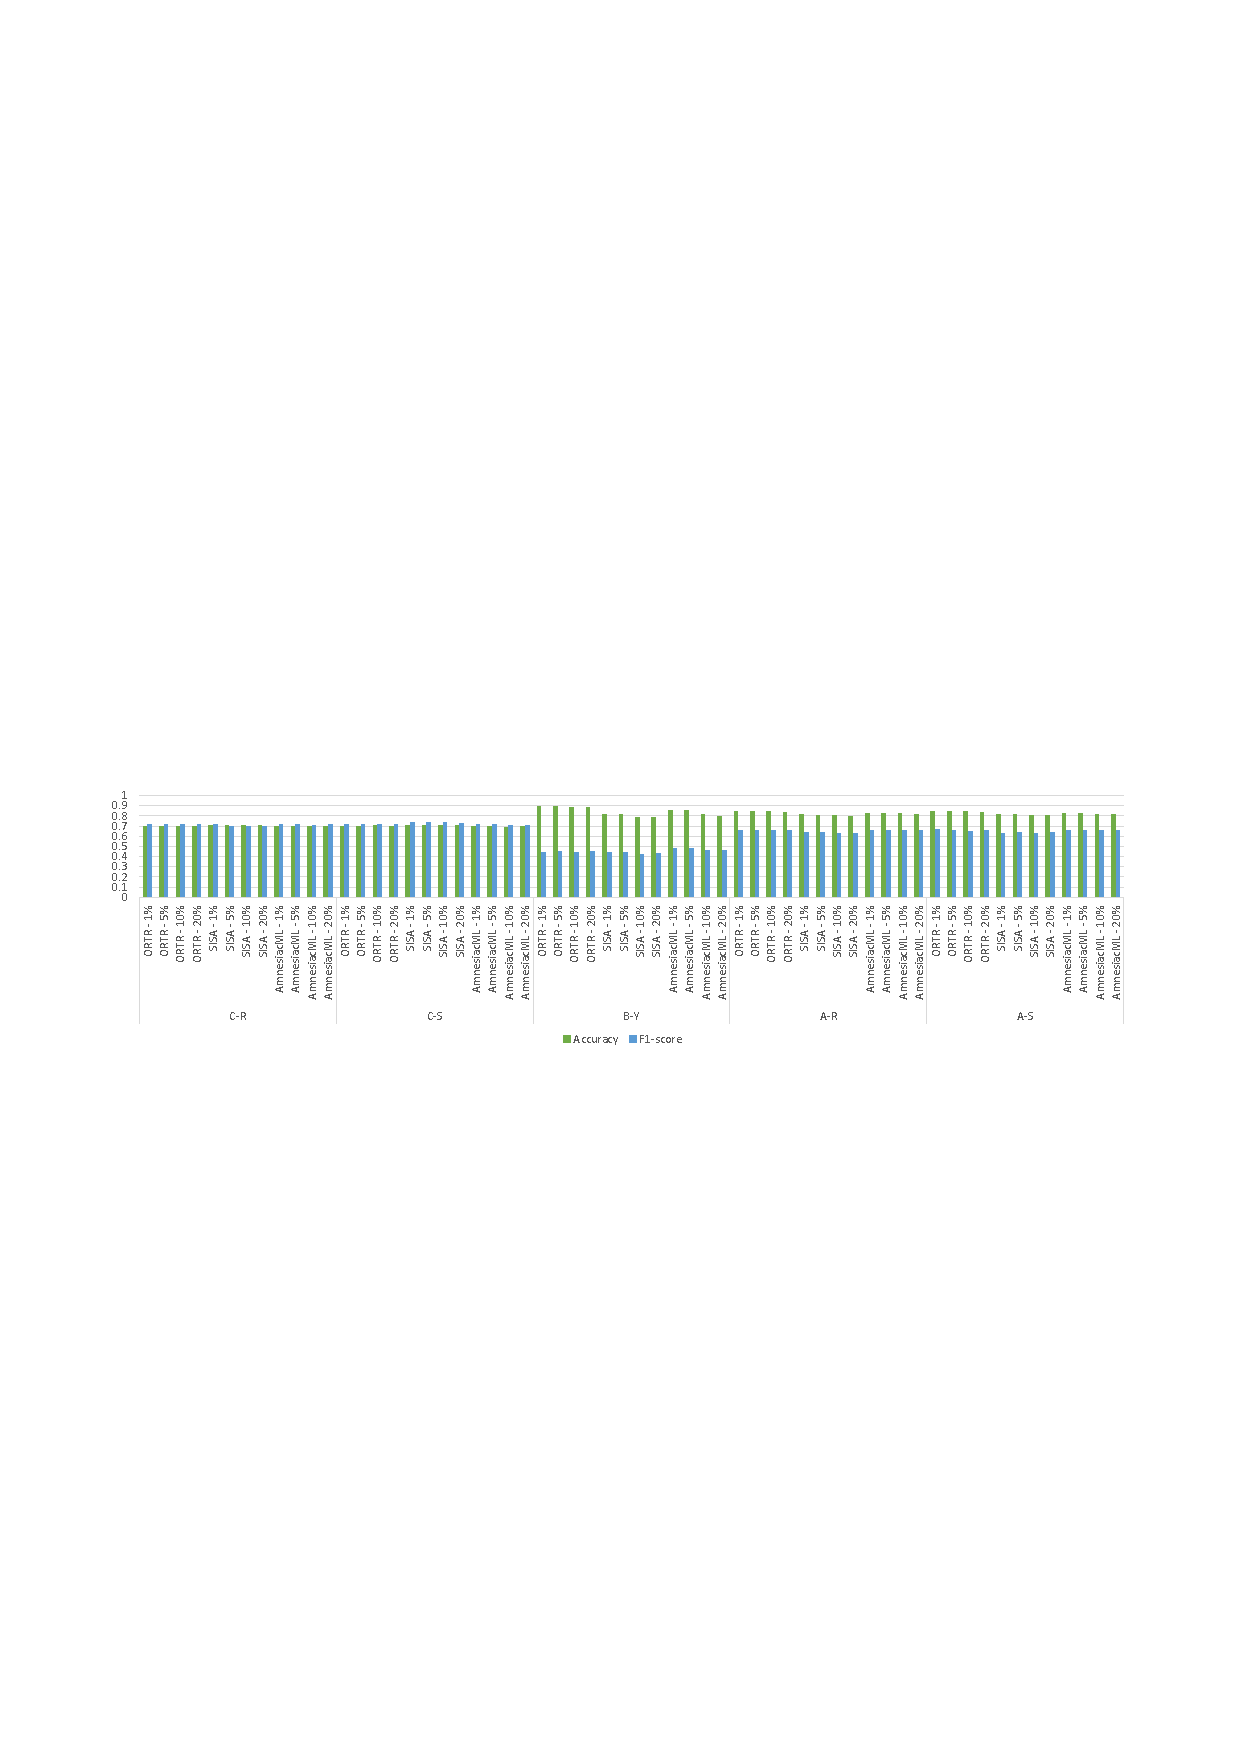
\includegraphics[width=1.0\textwidth]{assets/rq2-performance.pdf}
  \caption{Performance (the higher, the better) results of different training methods after uniform data deletion under various deletion proportions.}
  \label{fig:rq2-peformance}
 \vspace{-6pt}
\end{figure*}

Figure~\ref{fig:rq2-peformance} illustrates the performance of this data deletion strategy. It shows that the deleted data has minimal impact in terms of performance on trained models. As the deletion proportion is 1\% - 20\%, we believe the deleted data might be insufficient to cause non-trivial performance degradation.

\begin{tcolorbox}
Under the data deletion of uniform distribution, the fairness is not clearly affected by machine unlearning methods, while ORTR outperforms SISA and AmnesiacML on performance metrics.
\end{tcolorbox}


\begin{flushleft}
\textbf{RQ3: (Non-uniform distribution) What are the impacts of machine unlearning methods on fairness when the deleted data has non-uniform distribution?}
\end{flushleft}



People from different groups have the equal right to send RTBF requests to remove their sensitive information, but they may have varied probabilities~\cite{eurobarometer}. In this research question, we aim to understand the impacts of machine unlearning methods on fairness when the deleted data has non-uniform distribution. 



The simplest way to conduct the experiments is to remove the deleted data so that it has a similar distribution to the percentage of each group (privileged or unprivileged groups) for each sensitive feature on the whole dataset. As our datasets are imbalanced on some features, this RTBF simulation strategy highly likely leads to empty groups. To overcome this problem, we simplify our scenario by removing the data only from either the privileged group or the unprivileged group. Specifically, we remove 50\% of the data for each group, making the potential impact on fairness more apparent. Note that we assume the prior probability of a certain group (the privileged group or the unprivileged group) is known.



\begin{figure}[t!]
  \centering
  \begin{subfigure}[b]{0.48\textwidth}
  \centering
  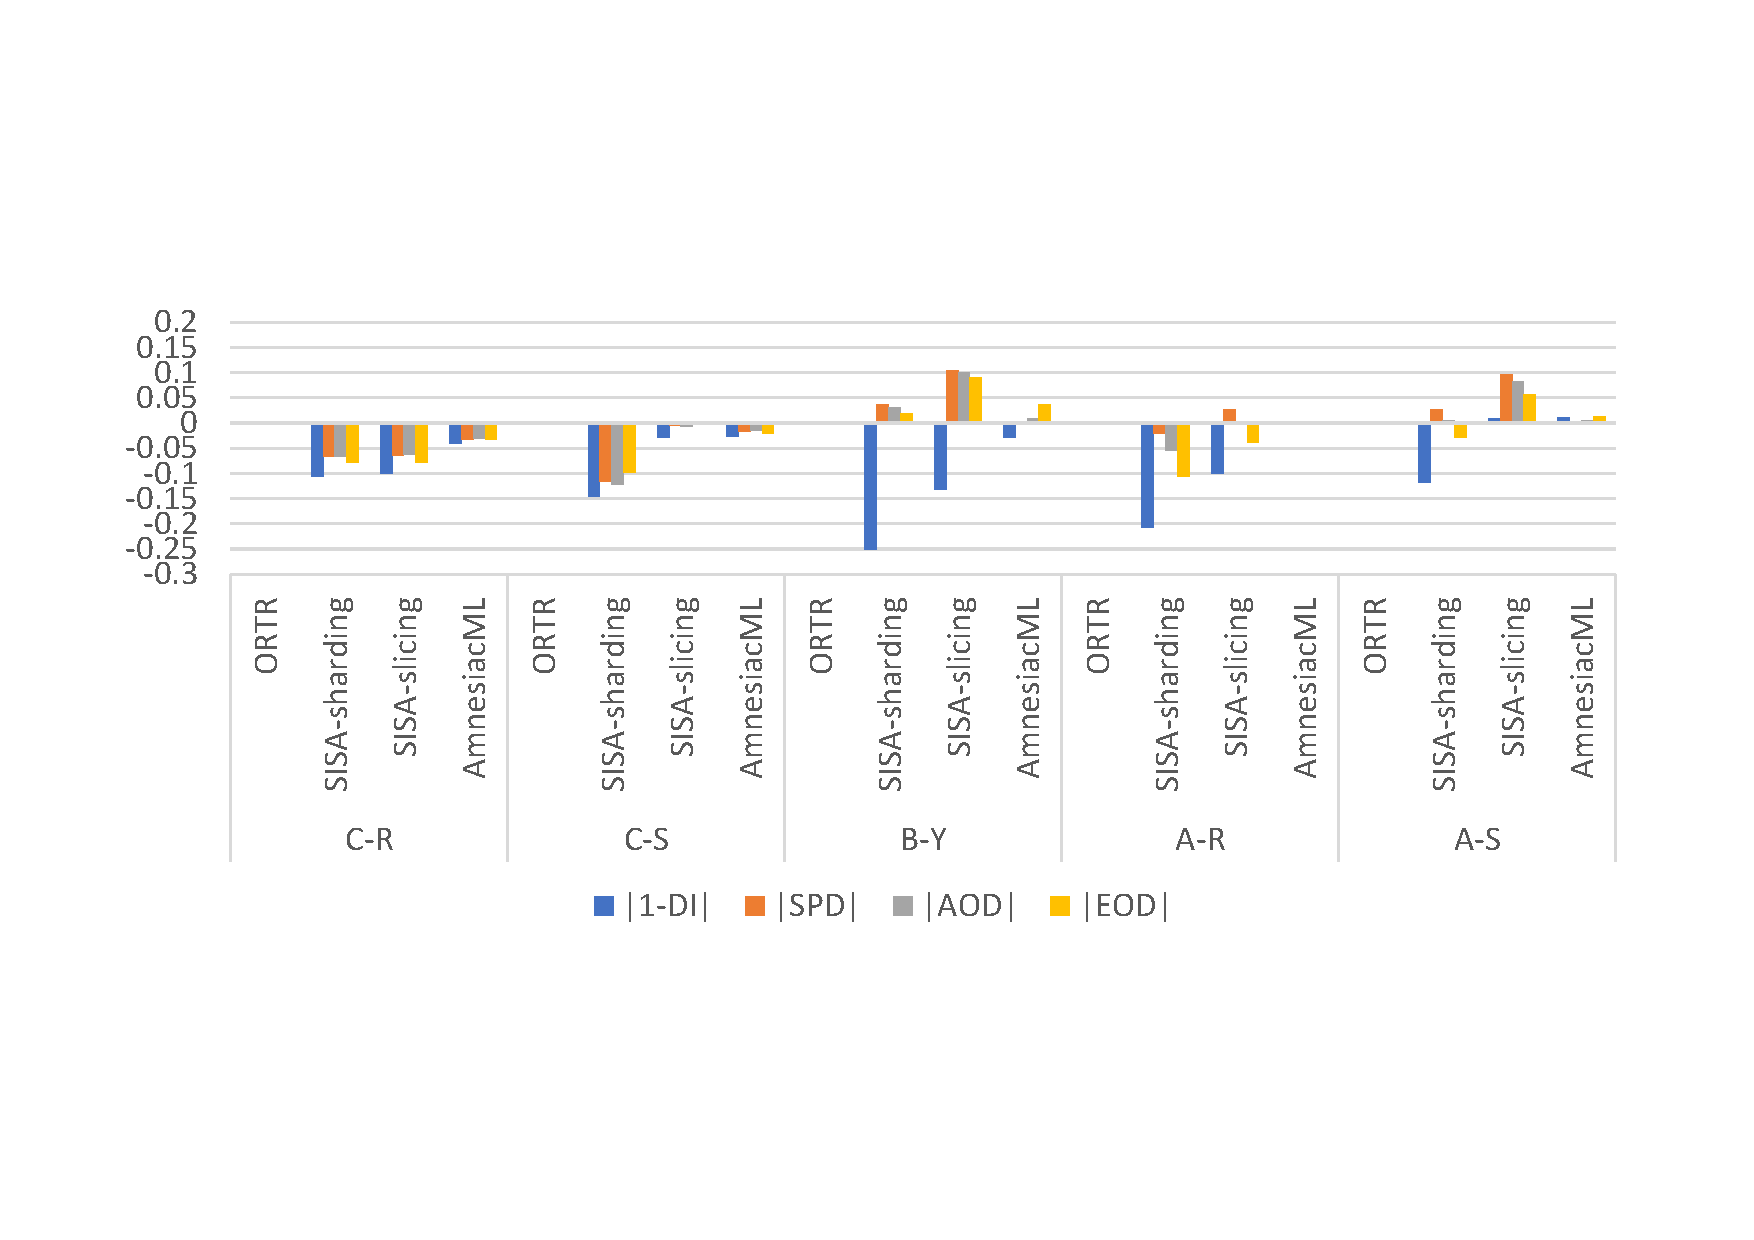
\includegraphics[width=\textwidth]{assets/rq3-fairness-privileged-diff.pdf}
  \caption{Fairness evaluation results after deletion from privileged group.}
  \label{fig:rq3-bar-chart-privileged}
  \end{subfigure}
  \begin{subfigure}[b]{0.48\textwidth}
  \centering
  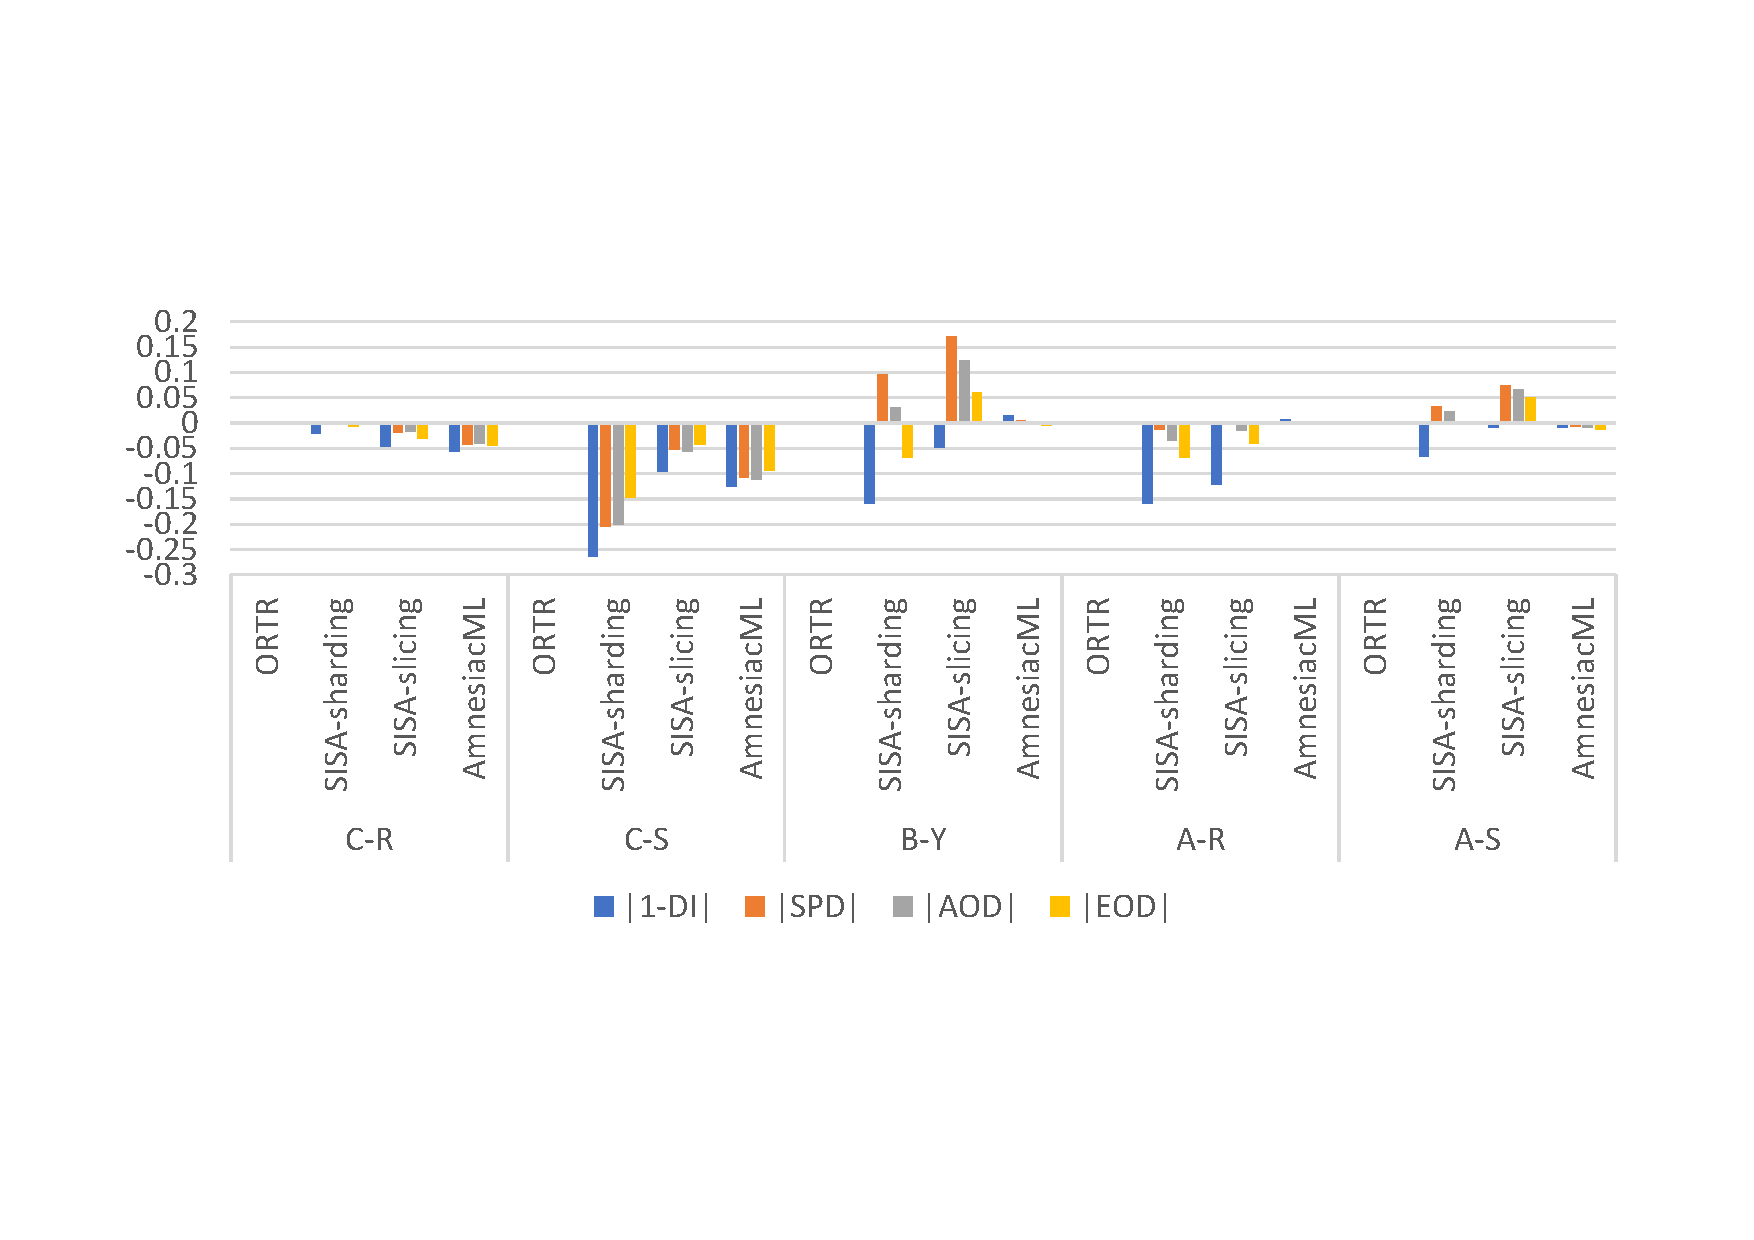
\includegraphics[width=\textwidth]{assets/rq3-fairness-unprivileged-diff.pdf}
  \caption{Fairness evaluation results after deletion from unprivileged group.}
  \label{fig:rq3-bar-chart-unprivileged}
  \end{subfigure}
  \caption{Fairness (the smaller, the better) evaluation results of non-uniform deletion. The results are shown as the distances from the ORTR results (baseline).}
  \label{fig:rq3-bar-chart}
 \vspace{-5pt}
\end{figure}



Figure~\ref{fig:rq3-bar-chart-privileged} and Figure~\ref{fig:rq3-bar-chart-unprivileged} present the results on data deletion from the privileged group and the unprivileged group, respectively.
From the charts we can see that SISA with a sharding strategy (see Figure~\ref{fig:sisa-sharding}) achieve the best $|1-\textrm{DI}|$ values for nine out of ten combinations. 
Figure~\ref{fig:rq3-before-after-deletion-diff} shows that SISA with a sharding strategy may also have fairness improvements after data deletion. The extent of improvements varies under different datasets, such as Adult, Bank, and COMPAS, and different sensitive features, i.e., \textit{Sex}, \textit{Race}, and \textit{Age}. Furthermore, we plot the differences between SISA with and without the sharding strategy in Figure~\ref{fig:rq3-with-without-sharding-strategy-diff}. Overall, the fairness is likely to be improved across all metrics when the sharding strategy is applied. Moreover, such improvements are likely to happen on those datasets and sensitive features with more imbalanced distributions.

\begin{figure}[t!]
  \centering
  \begin{subfigure}[b]{0.24\textwidth}
  \centering
  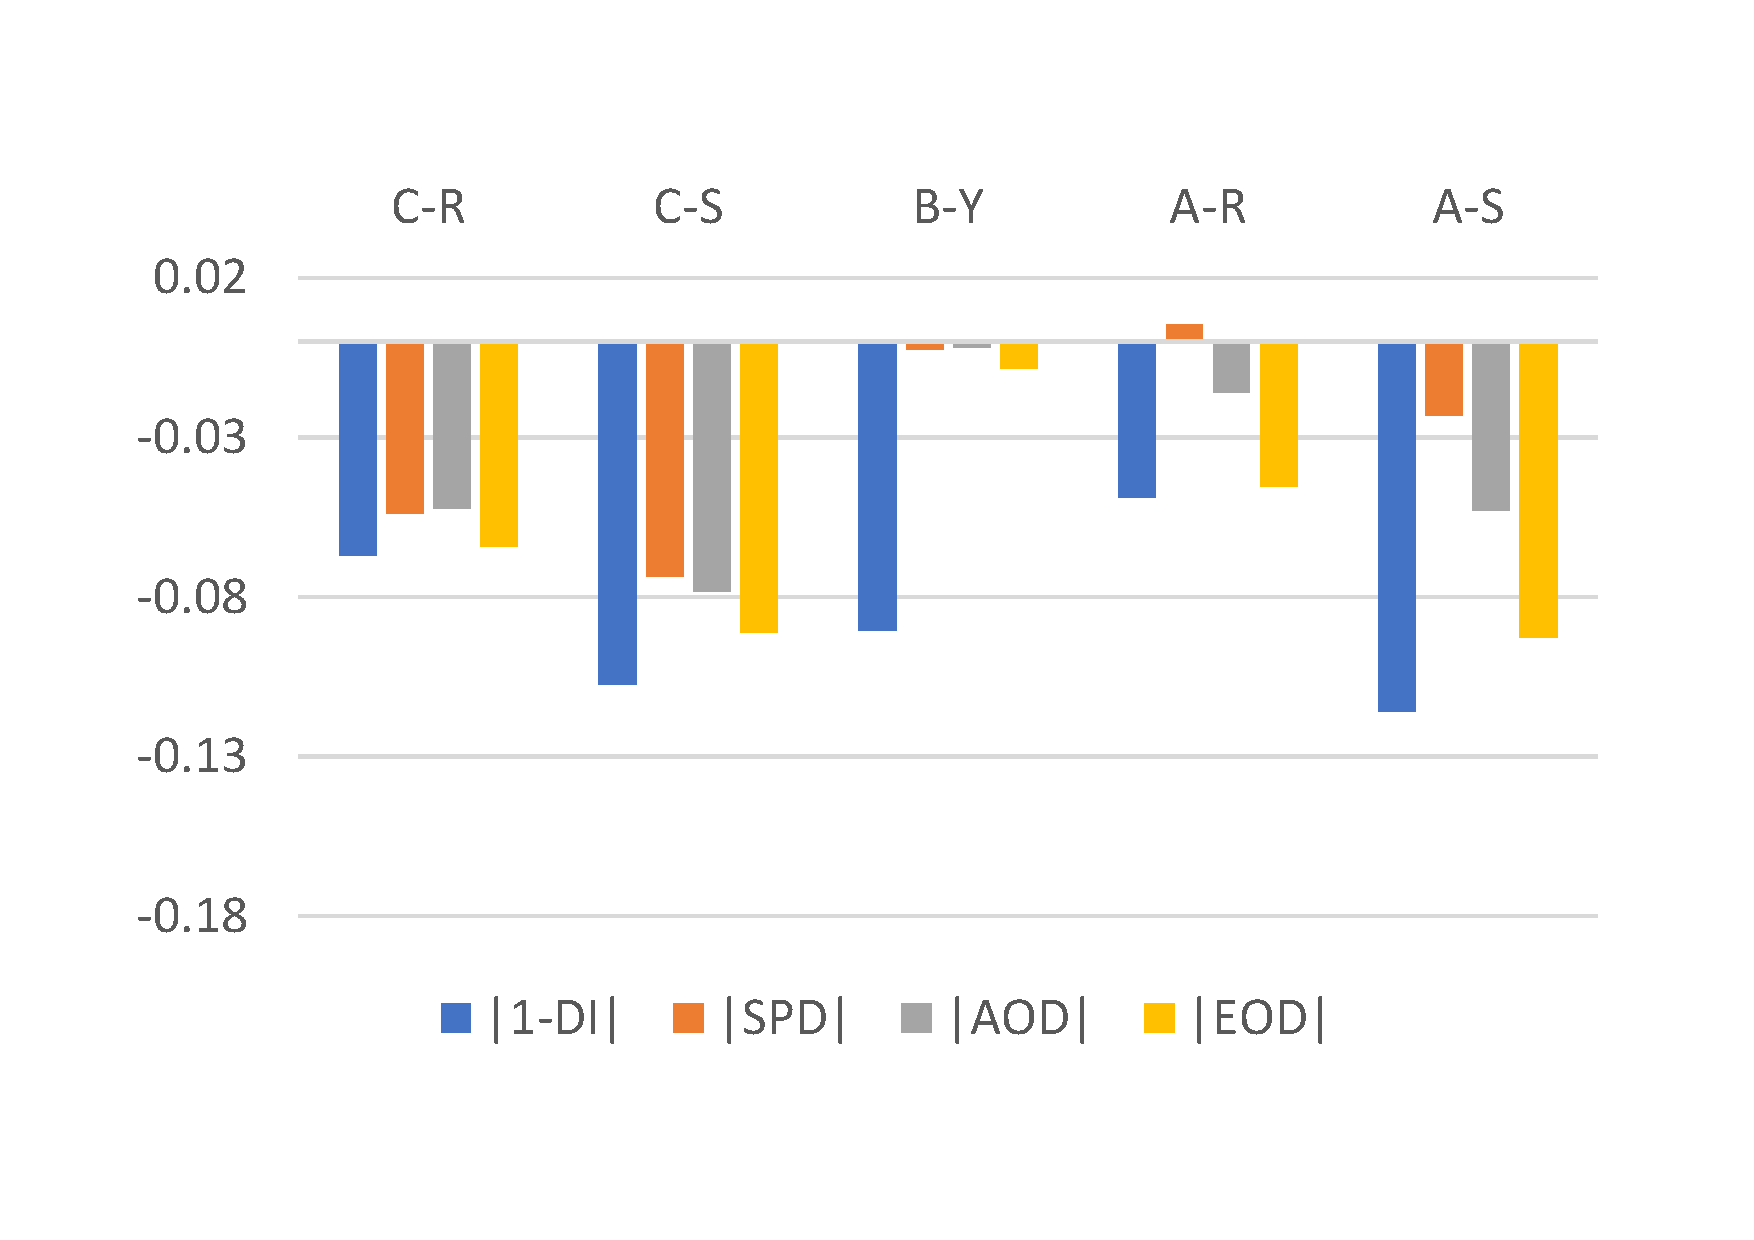
\includegraphics[width=\textwidth]{assets/rq3-before-after-deletion-privileged.pdf}
  \caption{Fairness change after deletion using SISA with sharding strategy on privileged groups.}
  \label{fig:rq3-before-after-deletion-privileged}
  \end{subfigure}
  \begin{subfigure}[b]{0.24\textwidth}
  \centering
  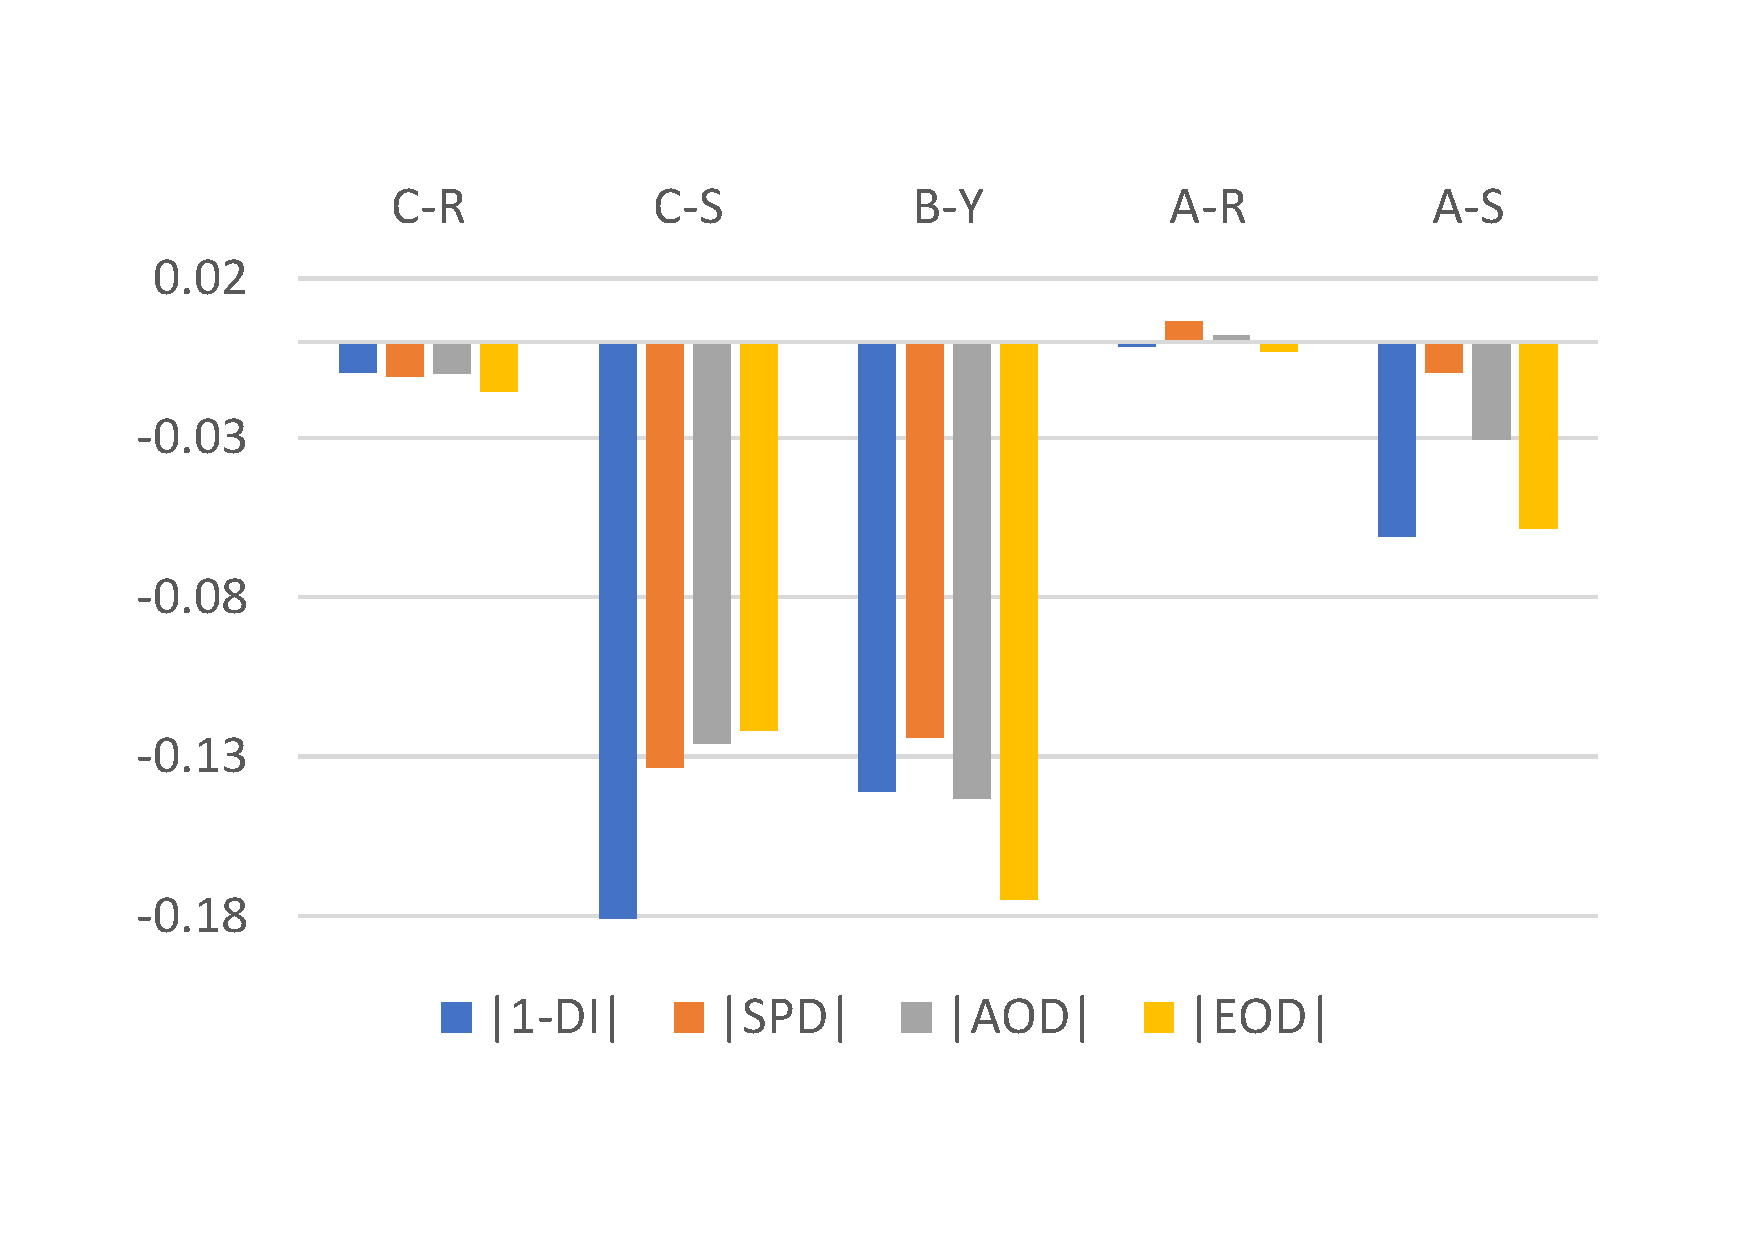
\includegraphics[width=\textwidth]{assets/rq3-before-after-deletion-unprivileged.pdf}
  \caption{Fairness change after deletion using SISA with sharding strategy on unprivileged groups.}
  \label{fig:rq3-before-after-deletion-unprivileged}
  \end{subfigure}
  \caption{Fairness change after deletion using SISA with sharding strategy.}
  \label{fig:rq3-before-after-deletion-diff}
\end{figure}




\begin{figure}[htbp!]
  \centering
  \begin{subfigure}[b]{0.24\textwidth}
  \centering
  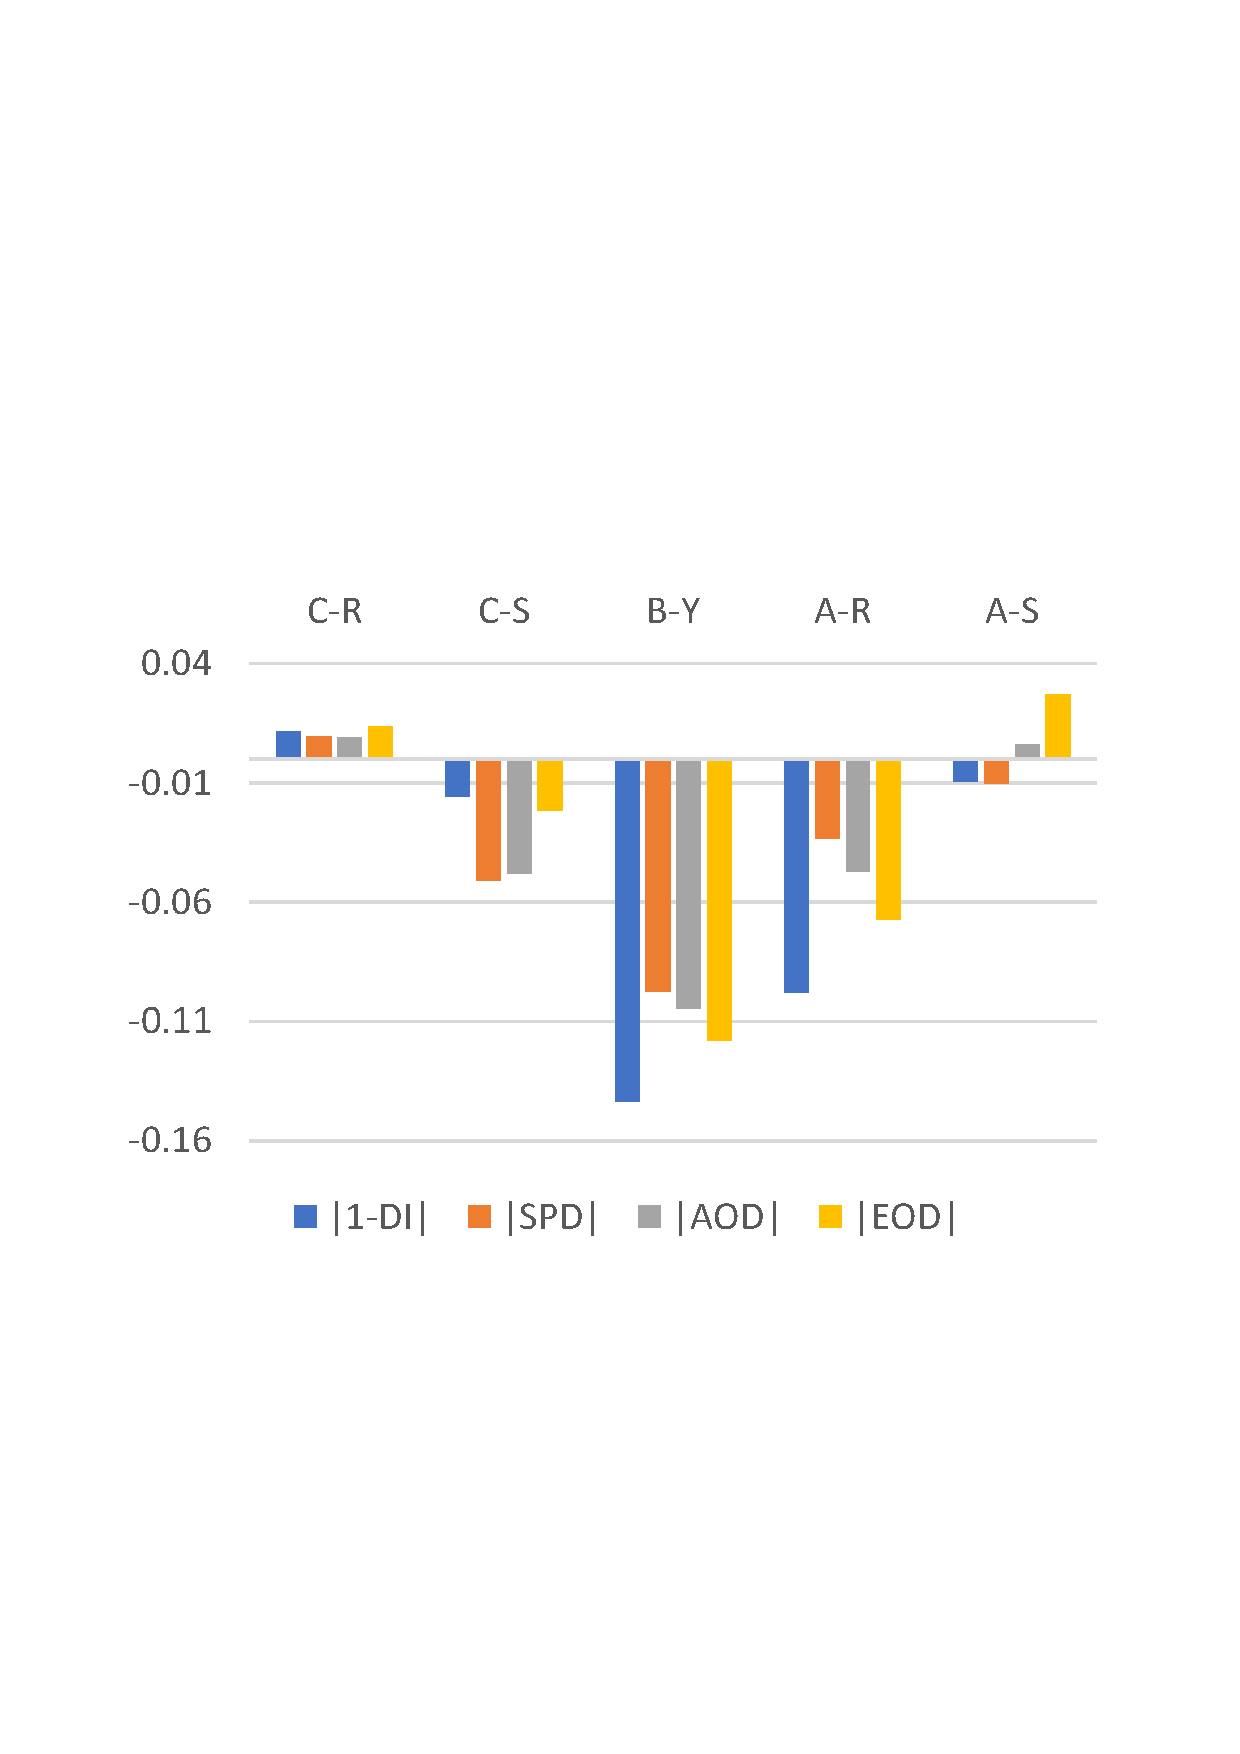
\includegraphics[width=\textwidth]{assets/rq3-with-without-sharding-strategy-diff-privileged.pdf}
  \caption{Fairness difference between SISA with and without applying sharding strategy on privileged groups.}
  \label{fig:rq3-with-without-sharding-strategy-diff-privileged}
  \end{subfigure}
  \begin{subfigure}[b]{0.24\textwidth}
  \centering
  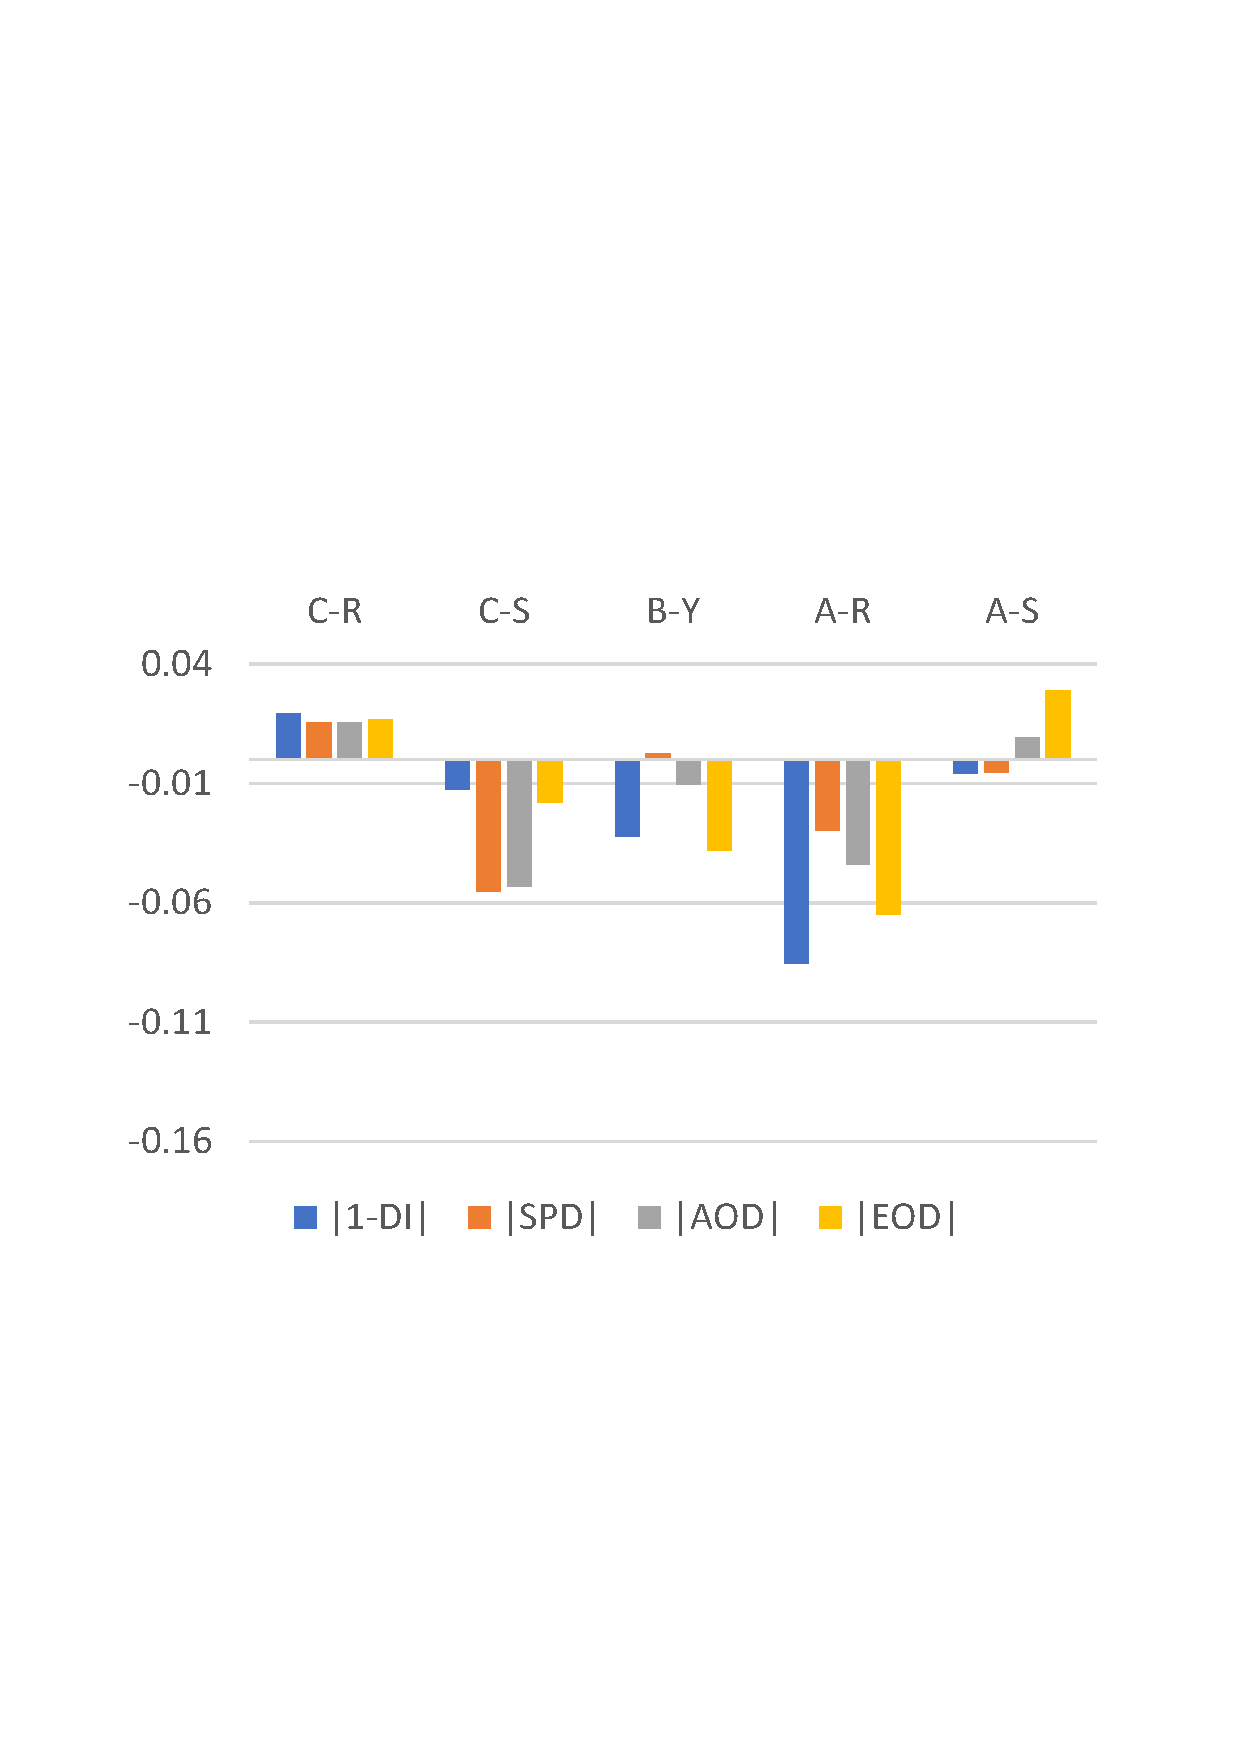
\includegraphics[width=\textwidth]{assets/rq3-with-without-sharding-strategy-diff-unprivileged.pdf}
  \caption{Fairness difference between SISA with and without applying sharding strategy on unprivileged groups.}
  \label{fig:rq3-with-without-sharding-strategy-diff-unprivileged}
  \end{subfigure}
  \caption{Fairness difference between SISA with and without applying sharding strategy.}
  \label{fig:rq3-with-without-sharding-strategy-diff}
\vspace{-5pt}
\end{figure}


SISA with a slicing strategy (see Figure~\ref{fig:sisa-slicing}) is also likely to outperform ORTR on $|1-\textrm{DI}|$. However, it achieves less performance compared to SISA with a sharding strategy. For ORTR, we observe that the fairness changes between before and after retraining are weak. Similarly, AmnesiacML tends to be close to the ORTR across all indicators. 

Performance-wise, we observed no significant performance difference between before and after the data deletion, or between methods with and without strategies applied. The changes in performance indicators are always less than 5\%. The performance differences between different methods are likely to be inherited from the methods instead of escalated from unlearning strategies or distribution settings.

\begin{tcolorbox}
Under the data deletion of non-uniform distribution, SISA with a sharding strategy achieves better fairness. The performance has no significant degradation from deletion using machine unlearning methods.
\end{tcolorbox}

